%%%%%%%%%%%%%%%%%%%%%%%%%%%%%%%%%%%%%%%%%%%%%%%%%%%%%%%%%%%%%%%%%%%%%%%%%%%%%
%% 03_arch_irq_concept.tex
%% Section: Interrupt Concept
%% Chapter: Architecture Concepts
%%
%% Describes the interrupt register structure inside every peripheral
%% (Service Request Block, shared RTL block as_irq_peripheral), the two
%% cases "different IRQs" and "IRQs of the same type", the interrupt flow
%% and the generic register description.
%% Same content as the HowTo PeripheralsIRQStructure/PerIRQ.tex.
%%
%% Integration in 00_rwurv64i_all.tex:
%%   \section{Interrupt Concept}
%%   \label{sec:archirq}
%%   \input{\TEXTarch 03_arch_history_tab03}
%%   \input{\TEXTarch 03_arch_irq_concept}
%%
%% Requires packages: tabularx, float, tikz, listings
%%   and the register macros \asregkopf, \asregfourxsixteen, \asregdesc
%%
%% v0.1  2026-11-18  Claude-AI  Initial version (from HowTo PerIRQ.tex)
%%%%%%%%%%%%%%%%%%%%%%%%%%%%%%%%%%%%%%%%%%%%%%%%%%%%%%%%%%%%%%%%%%%%%%%%%%%%%

% Timing diagrams: a signal is a path that alternates between low (y) and
% high (y+0.4) with |- , so every waypoint is "time, level".
\newcommand{\asirqwlabel}[2]{\node[anchor=east,font=\scriptsize] at (0,#1+0.2) {#2};}
\newcommand{\asirqwgrid}[1]{\foreach \t in {0,...,#1} \draw[very thin,lightgray] (\t,-0.2) -- (\t,6.2);}

%%%%%%%%%%%%%%%%%%%%%%%%%%%%%%%%%%%%%%%%%%%%%%%%%%%%%%%%%%%%%%%%%%%%%%%%%%%%%
\subsection{Introduction}
\label{subsec:archirqintro}
%%%%%%%%%%%%%%%%%%%%%%%%%%%%%%%%%%%%%%%%%%%%%%%%%%%%%%%%%%%%%%%%%%%%%%%%%%%%%

A peripheral kernel detects \textbf{events}: a pin changed, a byte was
received, the TX FIFO has space, a frame error occurred, \ldots{} An event is
only a pulse of one clock cycle, whereas software reacts much more slowly.
The event must therefore be \textbf{stored} until software has handled it.
Software must be able to
\begin{itemize}
  \item find out \textbf{which} event happened,
  \item \textbf{enable/disable} single events,
  \item \textbf{acknowledge} (clear) an event,
  \item \textbf{force} an event, to test the interrupt path without real hardware.
\end{itemize}
Every peripheral needs exactly this. Therefore all peripherals of the
\aschip use one \textbf{common interrupt register structure}, so that one
driver pattern fits all of them.

\paragraph{Origin.}
The structure is taken from the TOPSPIN peripheral architecture concepts
(2003). There, every bus peripheral contains a \textbf{Service Request Block
(SRB)}, which prepares the interrupt requests for the Interrupt Control Unit
(ICU) and the data transfer requests for the DMA controller. The basic register
set is RIS, IMSC, MIS, ICR and ISR (plus DMAE for DMA). For an interrupt with
several sources of the same type the set is extended by IRQSS, IRQSM and IRQSC.

\paragraph{Differences to TOPSPIN.}
\begin{itemize}
  \item \textbf{No DMA}: register DMAE and the data transfer request path are dropped.
  \item \textbf{64-bit registers}, one 8-byte aligned offset per register.
  \item \texttt{as\_irq\_peripheral} (in \texttt{ip\_irqper/src}) is one shared
    RTL block, used by GPIO0, UART0 and QSPI0.
  \item \textbf{Set wins over clear}: an event in the same clock cycle as a
    clear of the same bit is never lost.
  \item For sources of the same type, RIS[0] is \textbf{not stored a second
    time}: it is the level |(IRQSS\,\&\,IRQSM), so writing IRQSC is enough to
    clear the group interrupt.
  \item ICR, ISR and IRQSC are \textbf{write strobes}, not registers: they read 0.
\end{itemize}

\paragraph{Interrupt path on chip level.}
Figure~\ref{fig:archirq01} shows the complete path. This section describes the
interrupt registers inside each peripheral. ICU0 (Section~\ref{sec:icufunc01})
collects one line per peripheral (source 0\,=\,GPIO0, 1\,=\,UART0, 2\,=\,QSPI0)
and drives the machine external interrupt of the CPU
(\texttt{irq\_ext\_i[7]}, Section~\ref{subsec:irqconcept}).
\textbf{ICU0 latches the rising edge} of each peripheral line; this is
important for the interrupt flow (Section~\ref{subsec:archirqflow}).

\begin{figure}[H]
\centering
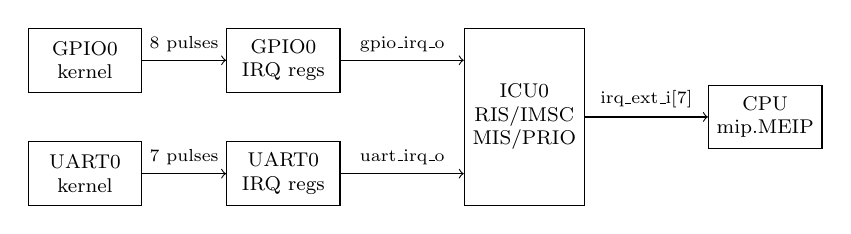
\begin{tikzpicture}[scale=0.9, transform shape,
    box/.style={draw, minimum height=0.9cm, minimum width=1.6cm, align=center, font=\footnotesize}]
  \node[box] (k1) at (0,1.2) {GPIO0\\kernel};
  \node[box] (s1) at (2.8,1.2) {GPIO0\\IRQ regs};
  \node[box] (k2) at (0,-0.4) {UART0\\kernel};
  \node[box] (s2) at (2.8,-0.4) {UART0\\IRQ regs};
  \node[box, minimum height=2.5cm] (icu) at (6.2,0.4) {ICU0\\RIS/IMSC\\MIS/PRIO};
  \node[box] (cpu) at (9.6,0.4) {CPU\\mip.MEIP};
  \draw[->] (k1) -- node[above,font=\scriptsize]{8 pulses} (s1);
  \draw[->] (k2) -- node[above,font=\scriptsize]{7 pulses} (s2);
  \draw[->] (s1) -- node[above,font=\scriptsize]{gpio\_irq\_o} (icu.west |- s1);
  \draw[->] (s2) -- node[above,font=\scriptsize]{uart\_irq\_o} (icu.west |- s2);
  \draw[->] (icu) -- node[above,font=\scriptsize]{irq\_ext\_i[7]} (cpu);
\end{tikzpicture}
\caption{Interrupt Path on Chip Level}
\label{fig:archirq01}
\end{figure}

%%%%%%%%%%%%%%%%%%%%%%%%%%%%%%%%%%%%%%%%%%%%%%%%%%%%%%%%%%%%%%%%%%%%%%%%%%%%%
\subsection{Interrupt Register Structure}
\label{subsec:archirqstruct}
%%%%%%%%%%%%%%%%%%%%%%%%%%%%%%%%%%%%%%%%%%%%%%%%%%%%%%%%%%%%%%%%%%%%%%%%%%%%%

Table~\ref{tab:archirq01} lists the interrupt register set. All write-1
registers act bit by bit: a 0 in the written data leaves the corresponding bit
unchanged. The interrupt output of the peripheral is \texttt{irq\_o\,=\,|MIS}.

\begin{table}[H]
\caption{Interrupt Register Set}
\label{tab:archirq01}
\centering
\begin{tabularx}{\textwidth}{|l|l|l|X|}
  \hline
  Name & Mode & Stored & Function \\
  \hline
  \hline
  RIS   & r  & yes & Raw Interrupt Status: 1 = event happened (pending) \\
  \hline
  IMSC  & rw & yes & Interrupt Mask Control: 1 = this RIS bit may raise the IRQ \\
  \hline
  MIS   & r  & no  & Masked Interrupt Status = RIS \& IMSC \\
  \hline
  ICR   & w  & no  & Interrupt Clear: writing 1 clears the RIS bit \\
  \hline
  ISR   & w  & no  & Interrupt Set: writing 1 sets the RIS bit (SW test) \\
  \hline
  \hline
  \multicolumn{4}{|l|}{\textit{only for IRQs of the same type}} \\
  \hline
  IRQSS & r  & yes & IRQ Source Status: one sticky bit per source \\
  \hline
  IRQSM & rw & yes & IRQ Source Mask: 1 = this source contributes to RIS[0] \\
  \hline
  IRQSC & w  & no  & IRQ Source Clear: writing 1 clears the IRQSS bit \\
  \hline
\end{tabularx}
\end{table}

Two cases are distinguished; \texttt{as\_irq\_peripheral} selects them with
the parameter \texttt{irqs\_yes\_no}:
\begin{description}
  \item[Different IRQs] (\texttt{irqs\_yes\_no}\,=\,0, e.g.\ UART0, QSPI0):
    every event has its own meaning (UART0: rx\_ready, tx\_ready, rx\_timeout,
    frame\_err, parity\_err, overrun\_err, break\_det). There is one RIS bit per
    event, \texttt{irq\_other\_i[n]} $\rightarrow$ RIS[$n$]. Registers: RIS,
    IMSC, MIS, ICR, ISR.
  \item[IRQs of the same type] (\texttt{irqs\_yes\_no}\,=\,1, e.g.\ GPIO0):
    many sources with the same meaning (``pin $k$ changed'', $k=0\ldots7$).
    There is one IRQSS bit per source, and the sources are ORed into
    \textbf{one} RIS bit:
    \texttt{irq\_same\_i[k]} $\rightarrow$ IRQSS[$k$] $\rightarrow$ RIS[0].
    The additional registers IRQSS, IRQSM and IRQSC exist. Different IRQs may
    exist next to the group: \texttt{irq\_other\_i[n]} $\rightarrow$ RIS[$n+1$].
\end{description}

\subsubsection{Different IRQs}
\label{subsubsec:archirqdiff}

Figure~\ref{fig:archirq02} shows the flow of one interrupt request bit $n$.
\begin{itemize}
  \item A pulse on \texttt{irq\_other\_i[n]} sets RIS[$n$].
  \item RIS[$n$] is \textbf{sticky}: it stays 1 until software writes a 1 to ICR[$n$].
  \item Software can set RIS[$n$] by writing a 1 to ISR[$n$].
  \item IMSC[$n$] decides whether RIS[$n$] reaches MIS[$n$] and the IRQ output.
  \item All bits of MIS are ORed: one IRQ line per peripheral to ICU0.
\end{itemize}

\begin{figure}[H]
\centering
\begin{tikzpicture}[scale=0.8, transform shape]
  \draw (0,0) rectangle (1,1);
  \node (RIS) at (0.5,1.25) {RIS};
  \draw (0,4) rectangle (1,5);
  \node (IMSC) at (0.5,5.25) {IMSC};
  \draw (4,4) rectangle (5,5);
  \node (MIS) at (4.5,5.25) {MIS};
  \draw (-2,1.5) -- (-1,1) -- (-1,0) -- (-2,-0.5) -- (-2,1.5);
  \draw (-5,0) rectangle (-4,1);
  \node (ISR) at (-4.5,1.25) {ISR};
  \draw (-5,-2) rectangle (-4,-1);
  \node (ICR) at (-4.5,-0.75) {ICR};
  \draw (2,2) rectangle (3,3);
  \node (AND) at (2.5,2.25) {\&};
  \draw[->] (-4,0.5) -- (-2,0.5);
  \draw (-4,-1.5) -- (-3,-1.5);
  \draw (-3,-1.5) -- (-3,0);
  \draw[->] (-3,0) -- (-2,0);
  \draw (-4,2.5) -- (-3,2.5);
  \draw (-3,2.5) -- (-3,1);
  \draw[->] (-3,1) -- (-2,1);
  \draw[->] (-1,0.5) -- (0,0.5);
  \draw (1,0.5) -- (1.5,0.5);
  \draw (1.5,0.5) -- (1.5,2.25);
  \draw[->] (1.5,2.25) -- (2,2.25);
  \draw (1,4.5) -- (1.5,4.5);
  \draw (1.5,4.5) -- (1.5,2.75);
  \draw[->] (1.5,2.75) -- (2,2.75);
  \draw[->] (3,2.5) -- (5,2.5);
  \draw (3.5, 2.5) -- (3.5,4.5);
  \draw[->] (3.5,4.5) -- (4,4.5);
  \node (IRQ1) at (-5,2.5) {IRQ Src};
  \node (IRQ2) at (6.5,2.5) {IRQ to ICU};
  \fill [black] (3.5,2.5) circle (0.1);
\end{tikzpicture}
\caption{Interrupt Request Flow (one bit $n$, different IRQs)}
\label{fig:archirq02}
\end{figure}

The core of the implementation in \texttt{as\_irq\_peripheral.sv}:
\begin{lstlisting}[basicstyle=\ttfamily\scriptsize]
ris_r <= (ris_r & ~ris_clr_s) | ris_set_s;  // set wins over clear
assign mis_s = ris_s & imsc_r;
assign irq_o = |mis_s;
\end{lstlisting}

\subsubsection{IRQs of the same Type}
\label{subsubsec:archirqsame}

Figure~\ref{fig:archirq03} shows the combination of several sources of the
same type into a single interrupt request (TOPSPIN).
\begin{itemize}
  \item A pulse on source $k$ sets IRQSS[$k$] (sticky).
  \item IRQSM[$k$] masks source $k$ \textbf{before} the OR.
  \item The OR of all unmasked pending sources forms the group request in RIS[0].
  \item IRQSC replaces ICR for the group: writing 1 to IRQSC[$k$] clears IRQSS[$k$].
    When no unmasked source is left, the group request is gone.
  \item TOPSPIN: a RIS bit forced via ISR is cleared by writing \textbf{any}
    IRQSC bit (the OR into the ICR path, grey ICR in the figure).
\end{itemize}

\begin{figure}[H]
\centering
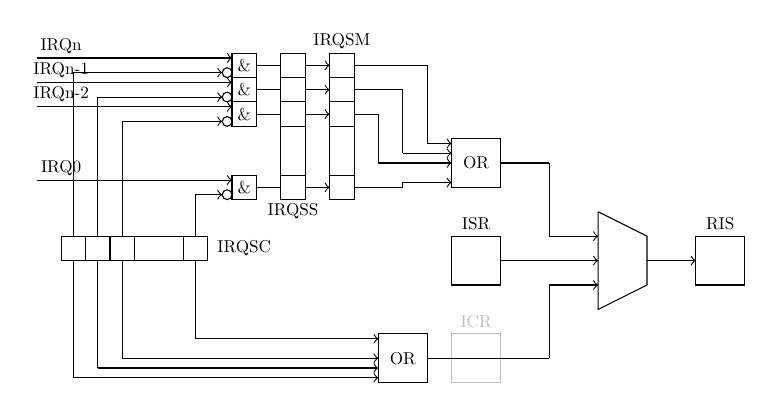
\begin{tikzpicture}[scale=0.62, transform shape]
  \draw (0,0) rectangle (1,1);
  \node (RIS) at (0.5,1.25) {RIS};
  \draw (-2,1.5) -- (-1,1) -- (-1,0) -- (-2,-0.5) -- (-2,1.5);
  \draw (-5,0) rectangle (-4,1);
  \node (ISR) at (-4.5,1.25) {ISR};
  \draw[draw=lightgray] (-5,-2) rectangle (-4,-1);
  \node[text=lightgray] (ICR) at (-4.5,-0.75) {ICR};
  \draw (-5,2) rectangle (-4,3);
  \node (OR1) at (-4.5,2.5) {OR};
  \draw (-6.5,-2) rectangle (-5.5,-1);
  \node (OR2) at (-6,-1.5) {OR};
  % IRQSM
  \draw (-7.5,1.75) rectangle (-7,2.25);
  \draw (-7.5,2.25) rectangle (-7,3.25);
  \draw (-7.5,3.25) rectangle (-7,3.75);
  \draw (-7.5,3.75) rectangle (-7,4.25);
  \draw (-7.5,4.25) rectangle (-7,4.75);
  % IRQSS
  \draw (-8.5,1.75) rectangle (-8,2.25);
  \draw (-8.5,2.25) rectangle (-8,3.25);
  \draw (-8.5,3.25) rectangle (-8,3.75);
  \draw (-8.5,3.75) rectangle (-8,4.25);
  \draw (-8.5,4.25) rectangle (-8,4.75);
  % IRQSC
  \draw (-10.5,0.5) rectangle (-10,1);
  \draw (-11.5,0.5) rectangle (-10.5,1);
  \draw (-12,0.5) rectangle (-11.5,1);
  \draw (-12.5,0.5) rectangle (-12,1);
  \draw (-13,0.5) rectangle (-12.5,1);
  % small ANDs with inverted input 1
  \draw (-9.5,1.75) rectangle (-9,2.25);
  \node at (-9.25,2.0) {\&};
  \draw (-9.6,1.85) circle (0.1);
  \draw (-9.5,3.25) rectangle (-9,3.75);
  \node at (-9.25,3.5) {\&};
  \draw (-9.6,3.35) circle (0.1);
  \draw (-9.5,3.75) rectangle (-9,4.25);
  \node at (-9.25,4) {\&};
  \draw (-9.6,3.85) circle (0.1);
  \draw (-9.5,4.25) rectangle (-9,4.75);
  \node at (-9.25,4.5) {\&};
  \draw (-9.6,4.35) circle (0.1);
  % Lines
  \draw[->] (-4,0.5) -- (-2,0.5);
  \draw (-4,-1.5) -- (-3,-1.5);
  \draw (-3,-1.5) -- (-3,0);
  \draw[->] (-3,0) -- (-2,0);
  \draw (-4,2.5) -- (-3,2.5);
  \draw (-3,2.5) -- (-3,1);
  \draw[->] (-3,1) -- (-2,1);
  \draw[->] (-1,0.5) -- (0,0.5);
  \draw (-7,2) -- (-6,2);
  \draw (-6,2) -- (-6,2.1);
  \draw[->] (-6,2.1) -- (-5,2.1);
  \draw (-7,3.5) -- (-6.5,3.5);
  \draw (-6.5,3.5) -- (-6.5,2.5);
  \draw[->] (-6.5,2.5) -- (-5,2.5);
  \draw (-7,4.0) -- (-6.0,4.0);
  \draw (-6.0,4.0) -- (-6.0,2.7);
  \draw[->] (-6.0,2.7) -- (-5,2.7);
  \draw (-7,4.5) -- (-5.5,4.5);
  \draw (-5.5,4.5) -- (-5.5,2.9);
  \draw[->] (-5.5,2.9) -- (-5,2.9);
  \draw (-5.5,-1.5) -- (-3.0,-1.5);
  \draw[->] (-8,2) -- (-7.5,2);
  \draw[->] (-8,3.5) -- (-7.5,3.5);
  \draw[->] (-8,4.0) -- (-7.5,4.0);
  \draw[->] (-8,4.5) -- (-7.5,4.5);
  \draw (-9,2) -- (-8.5,2);
  \draw (-9,3.5) -- (-8.5,3.5);
  \draw (-9,4.0) -- (-8.5,4.0);
  \draw (-9,4.5) -- (-8.5,4.5);
  \draw[->] (-13.5,2.15) -- (-9.5,2.15);
  \draw[->] (-13.5,3.65) -- (-9.5,3.65);
  \draw[->] (-13.5,4.15) -- (-9.5,4.15);
  \draw[->] (-13.5,4.65) -- (-9.5,4.65);
  \draw (-10.25,1.00) -- (-10.25,1.85);
  \draw[->] (-10.25,1.85) -- (-9.7,1.85);
  \draw (-11.75,1.00) -- (-11.75,3.35);
  \draw[->] (-11.75,3.35) -- (-9.7,3.35);
  \draw (-12.25,1.00) -- (-12.25,3.85);
  \draw[->] (-12.25,3.85) -- (-9.7,3.85);
  \draw (-12.75,1.00) -- (-12.75,4.35);
  \draw[->] (-12.75,4.35) -- (-9.7,4.35);
  \draw        (-10.25,0.50) -- (-10.25,-1.10);
  \draw[->] (-10.25,-1.10) -- (-6.50,-1.10);
  \draw        (-11.75,0.50) -- (-11.75,-1.50);
  \draw[->] (-11.75,-1.50) -- (-6.50,-1.50);
  \draw        (-12.25,0.50) -- (-12.25,-1.70);
  \draw[->] (-12.25,-1.70) -- (-6.50,-1.70);
  \draw        (-12.75,0.50) -- (-12.75,-1.90);
  \draw[->] (-12.75,-1.90) -- (-6.50,-1.90);
  \node at (-13.0,2.15+0.25) {IRQ0};
  \node at (-13.0,3.65+0.25) {IRQn-2};
  \node at (-13.0,4.15+0.25) {IRQn-1};
  \node at (-13.0,4.65+0.25) {IRQn};
  \node at (-7.25,4.75+0.25) {IRQSM};
  \node at (-8.25,1.5) {IRQSS};
  \node at (-9.25,0.75) {IRQSC};
\end{tikzpicture}
\caption{Interrupt Request with multiple Sources of the same Type}
\label{fig:archirq03}
\end{figure}

\paragraph{RWU-RV64I implementation.}
The \aschip simplifies the TOPSPIN structure: RIS[0] is not a second
flip-flop but RIS[0]\,=\,|(IRQSS\,\&\,IRQSM)\,|\,ris\_r[0]. IRQSC alone
therefore clears the group interrupt; ICR[0] only clears a bit 0 that was
forced by software via ISR. Signal flow and core of the implementation in
\texttt{as\_irq\_peripheral.sv}:
\begin{lstlisting}[basicstyle=\ttfamily\scriptsize]
  irq_same_i --> IRQSS --&--> OR --+
                 IRQSM --'         |
                                   v
  irq_other_i -------------------> RIS --&--> MIS --> OR --> irq_o
  ISR (write 1 = set) -----------> RIS    |
  ICR (write 1 = clear) ---------> RIS  IMSC

irqss_r <= (irqss_r & ~(wr_irqsc_s ? data_i : '0)) | irq_same_i;
assign irq_same_comb_s = |(irqss_r & irqsm_r);
assign ris_s = ris_r | {{(data_width-1){1'b0}}, irq_same_comb_s};
\end{lstlisting}
With \texttt{irqs\_yes\_no}\,=\,0 the registers IRQSS, IRQSM and IRQSC are not
built (generate) and their offsets are not decoded.

\subsubsection{Parameters of as\_irq\_peripheral}
\label{subsubsec:archirqparam}

\begin{table}[H]
\caption{Parameters of as\_irq\_peripheral}
\label{tab:archirq02}
\centering
\begin{tabularx}{\textwidth}{|l|X|l|l|l|}
  \hline
  Parameter & Meaning & GPIO0 & UART0 & QSPI0 \\
  \hline
  \hline
  irqs\_yes\_no   & 1: IRQSS, IRQSM, IRQSC exist & 1 & 0 & 0 \\
  \hline
  nr\_same\_irqs  & number of sources of the same type (IRQSS bits) & 8 & 1 (unused) & 1 (unused) \\
  \hline
  nr\_other\_irqs & number of different IRQs (RIS bits) & 1 (tied 0) & 7 & 5 \\
  \hline
  reg\_imsc\_rst  & reset value of IMSC & all 1 & 0 & 0 \\
  \hline
  reg\_irqsm\_rst & reset value of IRQSM & all 1 & -- & -- \\
  \hline
  addr\_offs\_*   & register offsets & 0x18--0x50 & 0x40--0x60 & 0x40--0x60 \\
  \hline
\end{tabularx}
\end{table}

The ports are \texttt{irq\_other\_i} and \texttt{irq\_same\_i} (pulses of one
clock cycle), \texttt{addr\_i}, \texttt{data\_i} and \texttt{en\_i} from the
slave BPI, and \texttt{data\_o}, \texttt{ris\_o} and \texttt{irq\_o}. The kernel
decides what an event is (edge, threshold, error); the block only stores the
pulse. ISR can only set the implemented RIS bits; all other RIS bits always read 0. The GPIO0 IMSC reset value ``all 1'' is temporary
(\texttt{as\_pack.sv}: ``change to 0 before tape-out'').

%%%%%%%%%%%%%%%%%%%%%%%%%%%%%%%%%%%%%%%%%%%%%%%%%%%%%%%%%%%%%%%%%%%%%%%%%%%%%
\subsection{Interrupt Flow}
\label{subsec:archirqflow}
%%%%%%%%%%%%%%%%%%%%%%%%%%%%%%%%%%%%%%%%%%%%%%%%%%%%%%%%%%%%%%%%%%%%%%%%%%%%%

\subsubsection{Different IRQs}
\label{subsubsec:archirqflowdiff}

\paragraph{Rules.}
\begin{itemize}
  \item An event sets its RIS bit, \textbf{independent of IMSC}.
  \item If an IMSC bit is disabled while its interrupt is active, the IRQ to the
    ICU is removed, but comes back when the IMSC bit is enabled again, unless
    RIS was cleared in the meantime.
  \item If the IMSC bit is not enabled when the event occurs, only RIS is set.
    Enabling IMSC later makes the interrupt active in MIS immediately.
  \item \textbf{Good practice}: before enabling an interrupt in IMSC, first clear
    the old RIS bit via ICR.
  \item If an event and an ICR write hit the same bit in the same clock cycle,
    \textbf{the bit stays set} (set wins over clear).
\end{itemize}

Figure~\ref{fig:archirq04} shows these rules for one RIS bit. In cycle 2 the
event arrives while the bit is masked; enabling IMSC in cycle 4 raises the IRQ.
In cycle 9 a new event and an ICR write coincide: RIS stays 1 and the second
interrupt is not lost.

\begin{figure}[H]
\centering
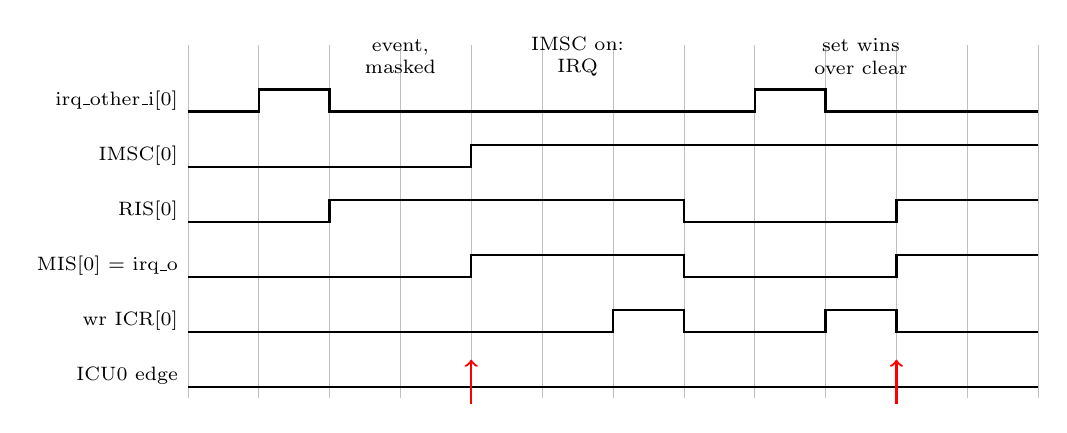
\begin{tikzpicture}[xscale=0.9, yscale=0.7]
  \asirqwgrid{12}
  \asirqwlabel{5}{irq\_other\_i[0]}
  \draw[thick] (0,5) -- (1,5) |- (2,5.4) |- (8,5) |- (9,5.4) |- (10,5) -- (12,5);
  \asirqwlabel{4}{IMSC[0]}
  \draw[thick] (0,4) -- (4,4) |- (12,4.4);
  \asirqwlabel{3}{RIS[0]}
  \draw[thick] (0,3) -- (2,3) |- (7,3.4) |- (10,3) |- (12,3.4);
  \asirqwlabel{2}{MIS[0] = irq\_o}
  \draw[thick] (0,2) -- (4,2) |- (7,2.4) |- (10,2) |- (12,2.4);
  \asirqwlabel{1}{wr ICR[0]}
  \draw[thick] (0,1) -- (6,1) |- (7,1.4) |- (9,1) |- (10,1.4) |- (12,1);
  \asirqwlabel{0}{ICU0 edge}
  \draw[thick] (0,0) -- (12,0);
  \foreach \t in {4,10} \draw[->,red,thick] (\t,-0.3) -- (\t,0.5);
  \node[font=\scriptsize,align=center] at (3,6.0) {event,\\masked};
  \node[font=\scriptsize,align=center] at (5.5,6.0) {IMSC on:\\IRQ};
  \node[font=\scriptsize,align=center] at (9.5,6.0) {set wins\\over clear};
\end{tikzpicture}
\caption{Timing of one RIS bit (different IRQs)}
\label{fig:archirq04}
\end{figure}

\paragraph{Software sequence (UART0).}
Initialisation: clear old events, then enable the wanted ones, then enable the
peripheral in ICU0 and the CPU.
\begin{lstlisting}[basicstyle=\ttfamily\scriptsize,language=C]
#define UART0      0x100000600UL
#define UART0_MIS  (*(volatile uint64_t *)(UART0 + 0x50))
#define UART0_IMSC (*(volatile uint64_t *)(UART0 + 0x48))
#define UART0_ICR  (*(volatile uint64_t *)(UART0 + 0x58))
#define RX_READY   (1UL << 0)
#define RX_TIMEOUT (1UL << 2)
#define ERR_ALL    (0xFUL << 3)   // frame, parity, overrun, break

UART0_ICR  = 0x7F;                            // 1. clear old events
UART0_IMSC = RX_READY | RX_TIMEOUT | ERR_ALL;  // 2. enable wanted ones
// 3. ICU0_IMSC bit 1, ICU0_CTRL.GIE, mie.MEIE, mstatus.MIE

void uart0_isr(void)
{
  uint64_t mis;
  ICU0_ICR = 1UL << 1;              // 0. ack ICU0 first
  while ((mis = UART0_MIS) != 0) {  // 1. which events?
    if (mis & (RX_READY | RX_TIMEOUT))
      read_rx_fifo();               // 2. read until empty
    if (mis & ERR_ALL)
      count_errors(mis);
    UART0_ICR = mis;                // 3. clear handled bits
  }
}
\end{lstlisting}
\begin{itemize}
  \item Clear only the bits that were read: an event that arrives during the
    service routine stays pending.
  \item Loop until MIS\,=\,0: \texttt{uart\_irq\_o} must fall, otherwise ICU0 never
    sees a new rising edge.
  \item Acknowledge ICU0\_ICR (\texttt{0x1\_0000\_0820}) \textbf{before} the loop,
    so that an edge after the loop is latched again and not lost.
\end{itemize}

\paragraph{Events derived from a level.}
Some events are conditions that last for a while (UART0: rx\_ready, tx\_ready,
rx\_timeout; QSPI0: all five sources). The kernel turns them into a pulse on the
\textbf{rising edge} of the condition, so RIS is set only once per edge. As long as
the condition stays true, clearing RIS does not produce a new event. Consequences
for software:
\begin{itemize}
  \item rx\_ready: the service routine must read the RX FIFO \textbf{below RXTHRES}
    (best: until it is empty). Otherwise no new rx\_ready interrupt comes; only
    rx\_timeout would fire later.
  \item tx\_ready: the service routine must fill the TX FIFO up to RXTHRES or more,
    so that the next fall below the threshold creates a new event.
  \item tx\_ready is set directly after reset (TX FIFO empty, level $<$ RXTHRES).
    This is the reason why the initialisation clears all RIS bits via ICR before it
    enables IMSC.
\end{itemize}

\subsubsection{IRQs of the same Type}
\label{subsubsec:archirqflowsame}

\paragraph{Rules.}
\begin{itemize}
  \item A pulse on a source sets its IRQSS bit, \textbf{independent of IRQSM}.
  \item IRQSM selects which sources form the group request; IMSC[0] enables the
    group as a whole.
  \item After reset \textbf{all sources are enabled} (IRQSM\,=\,all 1).
  \item The group request RIS[0] is a \textbf{level}: it stays 1 as long as at
    least one unmasked IRQSS bit is 1.
  \item Clearing: write 1s to IRQSC for the handled sources. ICR is not needed
    (only for a bit 0 forced via ISR).
  \item If an event and an IRQSC write hit the same bit in the same clock cycle,
    the IRQSS bit stays set.
\end{itemize}

Figure~\ref{fig:archirq05} shows a typical GPIO0 case. Pin 3 changes while
pin 0 is still pending, so ICU0 sees \textbf{no new edge}. After
IRQSC\,=\,0x01 the line is still high because of pin 3. The service routine
must therefore clear \textbf{all} pending sources before it returns.

\begin{figure}[H]
\centering
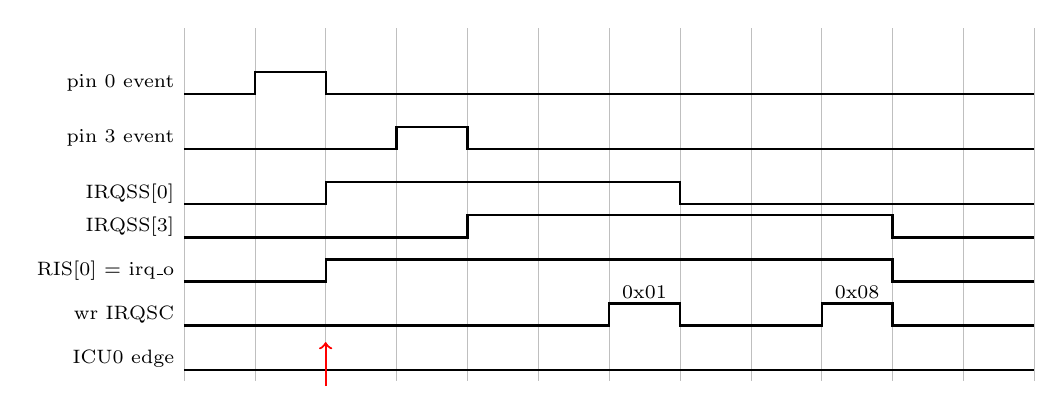
\begin{tikzpicture}[xscale=0.9, yscale=0.7]
  \asirqwgrid{12}
  \asirqwlabel{5}{pin 0 event}
  \draw[thick] (0,5) -- (1,5) |- (2,5.4) |- (12,5);
  \asirqwlabel{4}{pin 3 event}
  \draw[thick] (0,4) -- (3,4) |- (4,4.4) |- (12,4);
  \asirqwlabel{3}{IRQSS[0]}
  \draw[thick] (0,3) -- (2,3) |- (7,3.4) |- (12,3);
  \asirqwlabel{2.4}{IRQSS[3]}
  \draw[thick] (0,2.4) -- (4,2.4) |- (10,2.8) |- (12,2.4);
  \asirqwlabel{1.6}{RIS[0] = irq\_o}
  \draw[thick] (0,1.6) -- (2,1.6) |- (10,2.0) |- (12,1.6);
  \asirqwlabel{0.8}{wr IRQSC}
  \draw[thick] (0,0.8) -- (6,0.8) |- (7,1.2) |- (9,0.8) |- (10,1.2) |- (12,0.8);
  \node[font=\scriptsize] at (6.5,1.4) {0x01};
  \node[font=\scriptsize] at (9.5,1.4) {0x08};
  \asirqwlabel{0}{ICU0 edge}
  \draw[thick] (0,0) -- (12,0);
  \draw[->,red,thick] (2,-0.3) -- (2,0.5);
\end{tikzpicture}
\caption{Timing of a group of IRQs of the same type (GPIO0)}
\label{fig:archirq05}
\end{figure}

\paragraph{Software sequence (GPIO0).}
Initialisation: \texttt{GPIO0\_IRQSC\,=\,0xFF}, select the pins in
\texttt{GPIO0\_IRQSM}, then \texttt{GPIO0\_IMSC\,=\,1}, then enable source 0
in ICU0.
\begin{lstlisting}[basicstyle=\ttfamily\scriptsize,language=C]
#define GPIO0       0x100000000UL
#define GPIO0_IRQSS (*(volatile uint64_t *)(GPIO0 + 0x18))
#define GPIO0_IRQSM (*(volatile uint64_t *)(GPIO0 + 0x20))
#define GPIO0_IRQSC (*(volatile uint64_t *)(GPIO0 + 0x28))
#define GPIO0_MIS   (*(volatile uint64_t *)(GPIO0 + 0x48))

void gpio0_isr(void)
{
  uint64_t pins;
  ICU0_ICR = 1UL << 0;                // 0. ack ICU0 first
  while (GPIO0_MIS & 1) {             //    group active?
    pins = GPIO0_IRQSS & GPIO0_IRQSM; // 1. which pins?
    handle_pins(pins);                // 2. handle them
    GPIO0_IRQSC = pins;               // 3. clear sources
  }
}
\end{lstlisting}

\subsubsection{Comparison of both Cases}

\begin{table}[H]
\caption{Comparison: Different IRQs and IRQs of the same Type}
\label{tab:archirq03}
\centering
\begin{tabularx}{\textwidth}{|l|X|X|}
  \hline
   & Different IRQs (UART0) & Same type (GPIO0) \\
  \hline
  \hline
  Event stored in & RIS[$n$] & IRQSS[$k$] \\
  \hline
  Mask & IMSC[$n$] & IRQSM[$k$], then IMSC[0] \\
  \hline
  Which event? & read MIS & read IRQSS \& IRQSM \\
  \hline
  Clear & ICR[$n$] & IRQSC[$k$] \\
  \hline
  SW test & ISR[$n$] & ISR[0], clear with ICR[0] \\
  \hline
  RIS bit & sticky flip-flop & level |(IRQSS \& IRQSM) \\
  \hline
  Exit of service routine & loop until MIS\,=\,0 & loop until MIS[0]\,=\,0 \\
  \hline
\end{tabularx}
\end{table}

%%%%%%%%%%%%%%%%%%%%%%%%%%%%%%%%%%%%%%%%%%%%%%%%%%%%%%%%%%%%%%%%%%%%%%%%%%%%%
\subsection{Interrupt Register Description}
\label{subsec:archirqregs}
%%%%%%%%%%%%%%%%%%%%%%%%%%%%%%%%%%%%%%%%%%%%%%%%%%%%%%%%%%%%%%%%%%%%%%%%%%%%%

The following gives the generic description of the interrupt registers. The
peripheral sections define the offsets and the meaning of the single bits.

\paragraph{Read-Write Features.}
\begin{itemize}
  \item w: writable bit, by SW
  \item r: readable bit, by SW
  \item h: bit will be set by HW only
  \item X0: not implemented, reads 0
\end{itemize}

\paragraph{Parameters.}
\begin{itemize}
  \item \texttt{nr\_of\_irq}: number of RIS bits of the peripheral
    (UART0: 7; QSPI0: 5; GPIO0: 2, i.e.\ group bit 0 plus bit 1 for ISR only).
  \item \texttt{nr\_of\_irqs}: number of sources of the same type (GPIO0: 8).
  \item All registers are 64 bit wide; unused bits read 0.
\end{itemize}

\begin{table}[H]
\caption{Interrupt Register Offsets}
\label{tab:archirq04}
\centering
\begin{tabularx}{\textwidth}{|l|X|l|l|l|l|}
  \hline
  Symbol & Register Name & Mode & GPIO0 & UART0 & QSPI0 \\
  \hline
  \hline
  IRQSS & Interrupt Request Source Status & rh & 0x18 & -- & -- \\
  \hline
  IRQSM & Interrupt Request Source Mask   & rw & 0x20 & -- & -- \\
  \hline
  IRQSC & Interrupt Request Source Clear  & w  & 0x28 & -- & -- \\
  \hline
  ISR   & Interrupt Set                   & w  & 0x30 & 0x60 & 0x40 \\
  \hline
  RIS   & Raw Interrupt Status            & rh & 0x38 & 0x40 & 0x48 \\
  \hline
  IMSC  & Interrupt Mask Control          & rw & 0x40 & 0x48 & 0x50 \\
  \hline
  MIS   & Masked Interrupt Status         & rh & 0x48 & 0x50 & 0x58 \\
  \hline
  ICR   & Interrupt Clear                 & w  & 0x50 & 0x58 & 0x60 \\
  \hline
\end{tabularx}
\end{table}
Base addresses:
\begin{itemize}
  \item GPIO0: \texttt{0x1\_0000\_0000}
  \item QSPI0: \texttt{0x1\_0000\_0200} (RV\_PipelineCacheFwd only)
  \item UART0: \texttt{0x1\_0000\_0600}
\end{itemize}
The register names on chip level are \textbf{GPIO0\_RIS}, \textbf{UART0\_IMSC}, \ldots{}

\paragraph{RIS} -:
Raw Interrupt Status Register. Read-only. On a read it gives the current raw
status of each interrupt, independent of IMSC. Set by an event or by ISR,
cleared by ICR. A write has no effect.
\asregkopf{Raw Interrupt Status Register}{$0000000000000000_H$}
\asregfourxsixteen{\multicolumn{16}{|c|}{0}}
                  {\multicolumn{16}{|c|}{r}}
                  {\multicolumn{16}{|c|}{0}}
                  {\multicolumn{16}{|c|}{r}}
                  {\multicolumn{16}{|c|}{0}}
                  {\multicolumn{16}{|c|}{r}}
                  {\multicolumn{16}{|c|}{0 / RIS}}
                  {\multicolumn{16}{|c|}{r / rh}}
\asregdesc{RIS & nr\_of\_irq-1:0 & rh & One status bit per service request. 0: no interrupt, 1: interrupt pending. GPIO0: bit 0 = |(IRQSS \& IRQSM) or ISR-forced; bit 1 ISR-forced only. \\
           \hline
           0 & 63:nr\_of\_irq & r & Unimplemented, reserved}

\paragraph{IMSC} -:
Interrupt Mask Control Register. Read/write. A 1 enables, a 0 disables the
corresponding interrupt request. On a read it gives the current mask. The reset
value is defined per peripheral (UART0 and QSPI0: 0, GPIO0: all 1 until tape-out).
\asregkopf{Interrupt Mask Control Register}{$0000000000000000_H$}
\asregfourxsixteen{\multicolumn{16}{|c|}{0}}
                  {\multicolumn{16}{|c|}{r}}
                  {\multicolumn{16}{|c|}{0}}
                  {\multicolumn{16}{|c|}{r}}
                  {\multicolumn{16}{|c|}{0}}
                  {\multicolumn{16}{|c|}{r}}
                  {\multicolumn{16}{|c|}{0 / IMSC}}
                  {\multicolumn{16}{|c|}{r / rw}}
\asregdesc{IMSC & nr\_of\_irq-1:0 & rw & One mask bit per service request. 0: interrupt disabled, 1: interrupt enabled. \\
           \hline
           0 & 63:nr\_of\_irq & r & Unimplemented, reserved}

\paragraph{MIS} -:
Masked Interrupt Status Register. Read-only. On a read it gives the masked
status MIS\,=\,RIS\,\&\,IMSC (combinatorial, no flip-flop). The interrupt
output of the peripheral is |MIS. A write has no effect.
\asregkopf{Masked Interrupt Status Register}{$0000000000000000_H$}
\asregfourxsixteen{\multicolumn{16}{|c|}{0}}
                  {\multicolumn{16}{|c|}{r}}
                  {\multicolumn{16}{|c|}{0}}
                  {\multicolumn{16}{|c|}{r}}
                  {\multicolumn{16}{|c|}{0}}
                  {\multicolumn{16}{|c|}{r}}
                  {\multicolumn{16}{|c|}{0 / MIS}}
                  {\multicolumn{16}{|c|}{r / rh}}
\asregdesc{MIS & nr\_of\_irq-1:0 & rh & One masked status bit per service request. 0: no interrupt, 1: interrupt pending and enabled. \\
           \hline
           0 & 63:nr\_of\_irq & r & Unimplemented, reserved}

\paragraph{ICR} -:
Interrupt Clear Register. Write-only strobe, not stored. Writing a 1 clears the
corresponding RIS (and MIS) bit; a 0 has no effect. Reading returns 0. For a
group of the same type IRQSC replaces ICR; ICR[0] only clears a bit forced via
ISR.
\asregkopf{Interrupt Clear Register}{$0000000000000000_H$}
\asregfourxsixteen{\multicolumn{16}{|c|}{-}}
                  {\multicolumn{16}{|c|}{X0}}
                  {\multicolumn{16}{|c|}{-}}
                  {\multicolumn{16}{|c|}{X0}}
                  {\multicolumn{16}{|c|}{-}}
                  {\multicolumn{16}{|c|}{X0}}
                  {\multicolumn{16}{|c|}{- / ICR}}
                  {\multicolumn{16}{|c|}{X0 / w}}
\asregdesc{ICR & nr\_of\_irq-1:0 & w & One clear bit per service request. 0: no change, 1: clear interrupt. If set and clear hit the same bit in the same cycle, the set wins. Reading returns 0. \\
           \hline
           - & 63:nr\_of\_irq & X0 & Unimplemented, reserved}

\paragraph{ISR} -:
Interrupt Set Register. Write-only strobe, not stored. Writing a 1 sets the
corresponding RIS bit (and MIS if IMSC\,=\,1); a 0 has no effect. Reading
returns 0. Used to test the interrupt path without a real event.
\asregkopf{Interrupt Set Register}{$0000000000000000_H$}
\asregfourxsixteen{\multicolumn{16}{|c|}{-}}
                  {\multicolumn{16}{|c|}{X0}}
                  {\multicolumn{16}{|c|}{-}}
                  {\multicolumn{16}{|c|}{X0}}
                  {\multicolumn{16}{|c|}{-}}
                  {\multicolumn{16}{|c|}{X0}}
                  {\multicolumn{16}{|c|}{- / ISR}}
                  {\multicolumn{16}{|c|}{X0 / w}}
\asregdesc{ISR & nr\_of\_irq-1:0 & w & One set bit per service request. 0: no change, 1: set interrupt. Bits above nr\_of\_irq-1 are ignored. UART0: setting RIS[6:3] also sets STATUS[7:4]. Reading returns 0. \\
           \hline
           - & 63:nr\_of\_irq & X0 & Unimplemented, reserved}

\paragraph{IRQSS} -:
Interrupt Request Source Status Register. Read-only. One sticky bit per source
of the same type, set by the source pulse (GPIO0: an edge on the pin) and
cleared via IRQSC. A write has no effect. Only present if
\texttt{irqs\_yes\_no}\,=\,1.
\asregkopf{Interrupt Request Source Status Register (GPIO0: nr\_of\_irqs = 8)}{$0000000000000000_H$}
\asregfourxsixteen{\multicolumn{16}{|c|}{0}}
                  {\multicolumn{16}{|c|}{r}}
                  {\multicolumn{16}{|c|}{0}}
                  {\multicolumn{16}{|c|}{r}}
                  {\multicolumn{16}{|c|}{0}}
                  {\multicolumn{16}{|c|}{r}}
                  {\multicolumn{8}{|c|}{0}&\multicolumn{8}{c|}{IRQSS}}
                  {\multicolumn{8}{|c|}{r}&\multicolumn{8}{c|}{rh}}
\asregdesc{IRQSS & nr\_of\_irqs-1:0 & rh & One status bit per interrupt request source. 0: no request, 1: request pending. GPIO0: bit $k$ = edge on gpio\_io($k$). \\
           \hline
           0 & 63:nr\_of\_irqs & r & Unimplemented, reserved}

\paragraph{IRQSM} -:
Interrupt Request Source Mask Register. Read/write. A 1 enables, a 0 disables
the corresponding source before the OR into RIS[0]. On a read it gives the
current mask. After reset all sources are enabled. Only present if
\texttt{irqs\_yes\_no}\,=\,1.
\asregkopf{Interrupt Request Source Mask Register (GPIO0: nr\_of\_irqs = 8)}{$FFFFFFFFFFFFFFFF_H$}
\asregfourxsixteen{\multicolumn{16}{|c|}{IRQSM[63:48]}}
                  {\multicolumn{16}{|c|}{rw}}
                  {\multicolumn{16}{|c|}{IRQSM[47:32]}}
                  {\multicolumn{16}{|c|}{rw}}
                  {\multicolumn{16}{|c|}{IRQSM[31:16]}}
                  {\multicolumn{16}{|c|}{rw}}
                  {\multicolumn{8}{|c|}{IRQSM[15:8]}&\multicolumn{8}{c|}{IRQSM}}
                  {\multicolumn{8}{|c|}{rw}&\multicolumn{8}{c|}{rw}}
\asregdesc{IRQSM & nr\_of\_irqs-1:0 & rw & One mask bit per interrupt request source. 0: source disabled, 1: source enabled. \\
           \hline
           IRQSM & 63:nr\_of\_irqs & rw & Stored but without effect (no source connected)}

\paragraph{IRQSC} -:
Interrupt Request Source Clear Register. Write-only strobe, not stored.
Replaces ICR for the group. Writing a 1 clears the corresponding IRQSS bit; if
no further unmasked source is pending, RIS[0] and the IRQ drop in the same
cycle. Reading returns 0. Only present if \texttt{irqs\_yes\_no}\,=\,1.
\asregkopf{Interrupt Request Source Clear Register (GPIO0: nr\_of\_irqs = 8)}{$0000000000000000_H$}
\asregfourxsixteen{\multicolumn{16}{|c|}{-}}
                  {\multicolumn{16}{|c|}{X0}}
                  {\multicolumn{16}{|c|}{-}}
                  {\multicolumn{16}{|c|}{X0}}
                  {\multicolumn{16}{|c|}{-}}
                  {\multicolumn{16}{|c|}{X0}}
                  {\multicolumn{8}{|c|}{-}&\multicolumn{8}{c|}{IRQSC}}
                  {\multicolumn{8}{|c|}{X0}&\multicolumn{8}{c|}{w}}
\asregdesc{IRQSC & nr\_of\_irqs-1:0 & w & One clear bit per interrupt request source. 0: no change, 1: clear source. A source pulse in the same cycle wins. Reading returns 0. \\
           \hline
           - & 63:nr\_of\_irqs & X0 & Unimplemented, reserved}
